\documentclass[letterpaper]{article} % DO NOT CHANGE THIS
\usepackage[submission]{aaai2027}  % DO NOT CHANGE THIS
\usepackage[hyphens]{url}  % DO NOT CHANGE THIS
\usepackage{graphicx} % DO NOT CHANGE THIS
\urlstyle{rm} % DO NOT CHANGE THIS
\def\UrlFont{\rm}  % DO NOT CHANGE THIS
\usepackage{natbib}  % DO NOT CHANGE THIS AND DO NOT ADD ANY OPTIONS TO IT
\usepackage{caption} % DO NOT CHANGE THIS AND DO NOT ADD ANY OPTIONS TO IT
\frenchspacing  % DO NOT CHANGE THIS
\usepackage{booktabs}
\pdfinfo{
/TemplateVersion (2027.1)
}
\setcounter{secnumdepth}{2}

% Generated by analysis/make_tex.py; do not edit.
\newcommand{\nTestImages}{1{,}111}
\newcommand{\nTestObjects}{10{,}517}
\newcommand{\nSeaCucumber}{1{,}079}
\newcommand{\nSeaUrchin}{7{,}201}
\newcommand{\nScallop}{217}
\newcommand{\nStarfish}{2{,}020}
\newcommand{\shareSeaUrchin}{68}
\newcommand{\apYoloEightN}{0.624}
\newcommand{\ciYoloEightN}{[0.593, 0.655]}
\newcommand{\apYoloN}{0.625}
\newcommand{\ciYoloN}{[0.595, 0.652]}
\newcommand{\apYoloL}{0.690}
\newcommand{\ciYoloL}{[0.662, 0.716]}
\newcommand{\apGD}{0.090}
\newcommand{\ciGD}{[0.067, 0.114]}
\newcommand{\apGDtext}{0.048}
\newcommand{\ciGDtext}{[0.030, 0.069]}
\newcommand{\apOWL}{0.099}
\newcommand{\ciOWL}{[0.088, 0.111]}
\newcommand{\apQThree}{0.000}
\newcommand{\ciQThree}{[0.000, 0.000]}
\newcommand{\apQSeven}{0.013}
\newcommand{\ciQSeven}{[0.009, 0.018]}
\newcommand{\apGDlatin}{0.081}
\newcommand{\ciGDlatin}{[0.067, 0.100]}
\newcommand{\apOWLlatin}{0.086}
\newcommand{\ciOWLlatin}{[0.067, 0.105]}
\newcommand{\apQSevenLow}{0.007}
\newcommand{\ciQSevenLow}{[0.005, 0.015]}
\newcommand{\apQwenVL}{0.048}
\newcommand{\ciQwenVL}{[0.043, 0.056]}
\newcommand{\apHQwenVL}{0.054}
\newcommand{\ciHQwenVL}{[0.043, 0.087]}
\newcommand{\apHGD}{0.078}
\newcommand{\ciHGD}{[0.048, 0.138]}
\newcommand{\apHOWL}{0.107}
\newcommand{\ciHOWL}{[0.078, 0.140]}
\newcommand{\apHQSeven}{0.018}
\newcommand{\ciHQSeven}{[0.006, 0.034]}
\newcommand{\apHQThree}{0.000}
\newcommand{\ciHQThree}{[0.000, 0.000]}
\newcommand{\apHQSevenNoEmpty}{0.018}
\newcommand{\ciHQSevenNoEmpty}{[0.011, 0.030]}
\newcommand{\apHQThreeNoEmpty}{0.017}
\newcommand{\ciHQThreeNoEmpty}{[0.009, 0.032]}
\newcommand{\dGap}{+0.525}
\newcommand{\dciGap}{[0.493, 0.554]}
\newcommand{\dDecoding}{+0.042}
\newcommand{\dciDecoding}{[0.032, 0.053]}
\newcommand{\dOwlGd}{+0.009}
\newcommand{\dciOwlGd}{[$-$0.015, 0.031]}
\newcommand{\dLatinGd}{+0.009}
\newcommand{\dciLatinGd}{[$-$0.001, 0.016]}
\newcommand{\dLatinOwl}{+0.013}
\newcommand{\dciLatinOwl}{[0.001, 0.025]}
\newcommand{\dSevenThree}{+0.013}
\newcommand{\dciSevenThree}{[0.009, 0.018]}
\newcommand{\dResolution}{+0.005}
\newcommand{\dciResolution}{[$-$0.002, 0.009]}
\newcommand{\dYoloSize}{+0.065}
\newcommand{\dciYoloSize}{[0.056, 0.074]}
\newcommand{\dQwenGenFull}{+0.035}
\newcommand{\dciQwenGenFull}{[0.029, 0.043]}
\newcommand{\dOwlQwenFull}{+0.051}
\newcommand{\dciOwlQwenFull}{[0.040, 0.061]}
\newcommand{\dGdQwenFull}{+0.043}
\newcommand{\dciGdQwenFull}{[0.016, 0.064]}
\newcommand{\dQwenGen}{+0.036}
\newcommand{\dciQwenGen}{[0.021, 0.066]}
\newcommand{\dGdQwen}{+0.024}
\newcommand{\dciGdQwen}{[$-$0.014, 0.076]}
\newcommand{\dOwlQwen}{+0.053}
\newcommand{\dciOwlQwen}{[0.017, 0.078]}
\newcommand{\dPromptSeven}{+0.000}
\newcommand{\dciPromptSeven}{[$-$0.009, 0.011]}
\newcommand{\dPromptThree}{+0.017}
\newcommand{\dciPromptThree}{[0.009, 0.032]}
\newcommand{\rhoCocoDuo}{0.83}
\newcommand{\rhoCocoDuoCI}{[0.66, 0.94]}
\newcommand{\mgGD}{0.136}
\newcommand{\mgciGD}{[0.127, 0.146]}
\newcommand{\mgOWL}{0.151}
\newcommand{\mgciOWL}{[0.139, 0.164]}
\newcommand{\mgYoloN}{0.705}
\newcommand{\mgciYoloN}{[0.687, 0.725]}
\newcommand{\mgYoloL}{0.744}
\newcommand{\mgciYoloL}{[0.724, 0.763]}
\newcommand{\mgQSeven}{0.016}
\newcommand{\mgciQSeven}{[0.011, 0.019]}
\newcommand{\mgQwenVL}{0.083}
\newcommand{\mgciQwenVL}{[0.076, 0.094]}
\newcommand{\scApGD}{0.004}
\newcommand{\scApciGD}{[0.002, 0.008]}
\newcommand{\scApOWL}{0.001}
\newcommand{\scApciOWL}{[0.001, 0.002]}
\newcommand{\scApYoloN}{0.606}
\newcommand{\foundGD}{69}
\newcommand{\namedGD}{59}
\newcommand{\foundciGD}{[67, 72]}
\newcommand{\namedciGD}{[57, 61]}
\newcommand{\scFoundGD}{61}
\newcommand{\scNamedGD}{4}
\newcommand{\scFoundciGD}{[57, 65]}
\newcommand{\scNamedciGD}{[3, 6]}
\newcommand{\foundOWL}{62}
\newcommand{\namedOWL}{50}
\newcommand{\foundciOWL}{[59, 64]}
\newcommand{\namedciOWL}{[47, 52]}
\newcommand{\scFoundOWL}{52}
\newcommand{\scNamedOWL}{8}
\newcommand{\scFoundciOWL}{[49, 56]}
\newcommand{\scNamedciOWL}{[7, 10]}
\newcommand{\foundYoloN}{96}
\newcommand{\namedYoloN}{95}
\newcommand{\foundciYoloN}{[95, 97]}
\newcommand{\namedciYoloN}{[94, 96]}
\newcommand{\scFoundYoloN}{97}
\newcommand{\scNamedYoloN}{96}
\newcommand{\scFoundciYoloN}{[96, 98]}
\newcommand{\scNamedciYoloN}{[94, 97]}
\newcommand{\foundGDlatin}{59}
\newcommand{\namedGDlatin}{50}
\newcommand{\foundciGDlatin}{[57, 62]}
\newcommand{\namedciGDlatin}{[47, 52]}
\newcommand{\scFoundGDlatin}{52}
\newcommand{\scNamedGDlatin}{34}
\newcommand{\scFoundciGDlatin}{[49, 56]}
\newcommand{\scNamedciGDlatin}{[31, 39]}
\newcommand{\foundOWLlatin}{51}
\newcommand{\namedOWLlatin}{34}
\newcommand{\foundciOWLlatin}{[48, 54]}
\newcommand{\namedciOWLlatin}{[31, 36]}
\newcommand{\scFoundOWLlatin}{52}
\newcommand{\scNamedOWLlatin}{0}
\newcommand{\scFoundciOWLlatin}{[49, 56]}
\newcommand{\scNamedciOWLlatin}{[0, 0]}
\newcommand{\foundQwenVL}{44}
\newcommand{\namedQwenVL}{41}
\newcommand{\foundciQwenVL}{[42, 47]}
\newcommand{\namedciQwenVL}{[39, 43]}
\newcommand{\scFoundQwenVL}{15}
\newcommand{\scNamedQwenVL}{11}
\newcommand{\scFoundciQwenVL}{[13, 17]}
\newcommand{\scNamedciQwenVL}{[9, 13]}
\newcommand{\foundQSeven}{3}
\newcommand{\namedQSeven}{3}
\newcommand{\foundciQSeven}{[3, 4]}
\newcommand{\namedciQSeven}{[2, 4]}
\newcommand{\scFoundQSeven}{1}
\newcommand{\scNamedQSeven}{0}
\newcommand{\scFoundciQSeven}{[0, 1]}
\newcommand{\scNamedciQSeven}{[0, 1]}
\newcommand{\scUrchinGD}{574}
\newcommand{\scFoundNGD}{659}
\newcommand{\scStarOWL}{389}
\newcommand{\scFoundNOWL}{566}
\newcommand{\urchinAsHoloGDlatin}{1{,}260}
\newcommand{\urchinAsScalGDlatin}{1{,}014}
\newcommand{\urchinAsHoloGDlatinPct}{17}
\newcommand{\scStarOWLlatin}{517}
\newcommand{\starAsUrchinGD}{988}
\newcommand{\starAsStarGD}{421}
\newcommand{\scalAsStarOWL}{87}
\newcommand{\scalAsUrchinOWL}{79}
\newcommand{\scalAsScalOWL}{16}
\newcommand{\scNamedTopTenGD}{0}
\newcommand{\scFoundTopTenGD}{21}
\newcommand{\scNamedIouSeventyGD}{4}
\newcommand{\scFoundIouSeventyGD}{49}
\newcommand{\scNamedTopTenOWL}{3}
\newcommand{\scFoundTopTenOWL}{20}
\newcommand{\scNamedIouSeventyOWL}{5}
\newcommand{\scFoundIouSeventyOWL}{31}
\newcommand{\bPQwenVL}{0.349}
\newcommand{\bRQwenVL}{0.402}
\newcommand{\bPciQwenVL}{[0.327, 0.374]}
\newcommand{\bRciQwenVL}{[0.382, 0.424]}
\newcommand{\bBoxesQwenVL}{10.9}
\newcommand{\bPGD}{0.236}
\newcommand{\bRGD}{0.273}
\newcommand{\bPciGD}{[0.220, 0.252]}
\newcommand{\bRciGD}{[0.256, 0.289]}
\newcommand{\bBoxesGD}{10.9}
\newcommand{\bPOWL}{0.349}
\newcommand{\bROWL}{0.341}
\newcommand{\bPciOWL}{[0.323, 0.377]}
\newcommand{\bRciOWL}{[0.321, 0.360]}
\newcommand{\bBoxesOWL}{9.2}
\newcommand{\bPYoloN}{0.558}
\newcommand{\bRYoloN}{0.624}
\newcommand{\bPciYoloN}{[0.525, 0.591]}
\newcommand{\bRciYoloN}{[0.594, 0.653]}
\newcommand{\bBoxesYoloN}{10.6}
\newcommand{\bdPGD}{+0.112}
\newcommand{\bdciPGD}{[0.099, 0.127]}
\newcommand{\bdRGD}{+0.130}
\newcommand{\bdciRGD}{[0.117, 0.144]}
\newcommand{\bdPOWL}{$-$0.001}
\newcommand{\bdciPOWL}{[$-$0.016, 0.016]}
\newcommand{\bdROWL}{+0.061}
\newcommand{\bdciROWL}{[0.048, 0.076]}
\newcommand{\nRepQThree}{1{,}111}
\newcommand{\nEmptyQThree}{1{,}111}
\newcommand{\nCutQThree}{0}
\newcommand{\nRepQSeven}{1{,}111}
\newcommand{\nEmptyQSeven}{1{,}005}
\newcommand{\nCutQSeven}{0}
\newcommand{\nRepQThreeNoEmpty}{100}
\newcommand{\nEmptyQThreeNoEmpty}{0}
\newcommand{\nCutQThreeNoEmpty}{4}
\newcommand{\nRepQSevenNoEmpty}{100}
\newcommand{\nEmptyQSevenNoEmpty}{0}
\newcommand{\nCutQSevenNoEmpty}{18}
\newcommand{\nRepQwenVL}{1{,}111}
\newcommand{\nEmptyQwenVL}{177}
\newcommand{\nCutQwenVL}{229}
\newcommand{\nRepQSevenLow}{1{,}111}
\newcommand{\nEmptyQSevenLow}{1{,}017}
\newcommand{\nCutQSevenLow}{6}
\newcommand{\pctEmptyQSeven}{90}
\newcommand{\nUnmatchedText}{4{,}633}
\newcommand{\nBoxesText}{14{,}427}
\newcommand{\pctUnmatchedText}{32}
\newcommand{\nOutsideQwenVL}{374}
\newcommand{\secQwenVLmean}{15.8}
\newcommand{\secQwenVLmedian}{7.9}
\newcommand{\nImagesWithObjects}{1{,}100}
\newcommand{\lossNamingGD}{10}
\newcommand{\lossNamingOWL}{12}
\newcommand{\mgYoloEightN}{0.700}
\newcommand{\namedOfFoundMinYoloN}{97}
\newcommand{\namedOfFoundMaxYoloN}{100}
\newcommand{\trainMinMinutes}{27}
\newcommand{\trainMaxMinutes}{155}
\newcommand{\secOWL}{0.3}
\newcommand{\secQSeven}{0.6}
\newcommand{\gtbPGD}{0.299}
\newcommand{\gtbRGD}{0.299}
\newcommand{\gtbPOWL}{0.429}
\newcommand{\gtbROWL}{0.384}
\newcommand{\gtbPYoloN}{0.861}
\newcommand{\gtbRYoloN}{0.861}
\newcommand{\nCrops}{1{,}117}
\newcommand{\nCropsScallop}{217}
\newcommand{\nCropsOther}{300}
\newcommand{\cropGD}{28}
\newcommand{\cropciGD}{[27, 29]}
\newcommand{\cropDefaultGD}{95}
\newcommand{\cropCucGD}{0}
\newcommand{\cropUrchGD}{98}
\newcommand{\cropScalGD}{3}
\newcommand{\cropStarGD}{10}
\newcommand{\cropOWL}{26}
\newcommand{\cropciOWL}{[25, 27]}
\newcommand{\cropDefaultOWL}{91}
\newcommand{\cropCucOWL}{2}
\newcommand{\cropUrchOWL}{8}
\newcommand{\cropScalOWL}{1}
\newcommand{\cropStarOWL}{92}
\newcommand{\cropQThree}{33}
\newcommand{\cropciQThree}{[31, 35]}
\newcommand{\cropDefaultQThree}{57}
\newcommand{\cropCucQThree}{47}
\newcommand{\cropUrchQThree}{69}
\newcommand{\cropScalQThree}{6}
\newcommand{\cropStarQThree}{9}
\newcommand{\cropQSeven}{33}
\newcommand{\cropciQSeven}{[30, 35]}
\newcommand{\cropDefaultQSeven}{59}
\newcommand{\cropCucQSeven}{62}
\newcommand{\cropUrchQSeven}{40}
\newcommand{\cropScalQSeven}{16}
\newcommand{\cropStarQSeven}{13}
\newcommand{\cropQwenVL}{48}
\newcommand{\cropciQwenVL}{[45, 50]}
\newcommand{\cropDefaultQwenVL}{52}
\newcommand{\cropCucQwenVL}{71}
\newcommand{\cropUrchQwenVL}{50}
\newcommand{\cropScalQwenVL}{12}
\newcommand{\cropStarQwenVL}{58}
\newcommand{\cropGDlatin}{28}
\newcommand{\cropciGDlatin}{[26, 30]}
\newcommand{\cropDefaultGDlatin}{88}
\newcommand{\cropCucGDlatin}{88}
\newcommand{\cropUrchGDlatin}{5}
\newcommand{\cropScalGDlatin}{7}
\newcommand{\cropStarGDlatin}{13}
\newcommand{\cropOWLlatin}{28}
\newcommand{\cropciOWLlatin}{[26, 30]}
\newcommand{\cropDefaultOWLlatin}{65}
\newcommand{\cropCucOWLlatin}{25}
\newcommand{\cropUrchOWLlatin}{7}
\newcommand{\cropScalOWLlatin}{3}
\newcommand{\cropStarOWLlatin}{76}
\newcommand{\cropScalMax}{16}
\newcommand{\cropdGD}{+20}
\newcommand{\cropdciGD}{[18, 23]}
\newcommand{\cropdOWL}{+22}
\newcommand{\cropdciOWL}{[19, 25]}
\newcommand{\cropdQSeven}{+15}
\newcommand{\cropdciQSeven}{[12, 18]}
\newcommand{\msYoloMin}{10}
\newcommand{\msYoloMax}{21}
\newcommand{\rApYoloEightN}{0.582}
\newcommand{\rApciYoloEightN}{[0.573, 0.594]}
\newcommand{\rSeaYoloEightN}{0.481}
\newcommand{\rSeaciYoloEightN}{[0.469, 0.492]}
\newcommand{\rOthYoloEightN}{0.650}
\newcommand{\rOthciYoloEightN}{[0.635, 0.669]}
\newcommand{\rFoundSeaYoloEightN}{96}
\newcommand{\rNamedSeaYoloEightN}{94}
\newcommand{\rFoundciSeaYoloEightN}{[95, 96]}
\newcommand{\rNamedciSeaYoloEightN}{[94, 95]}
\newcommand{\rFoundOthYoloEightN}{95}
\newcommand{\rNamedOthYoloEightN}{94}
\newcommand{\rFoundciOthYoloEightN}{[92, 96]}
\newcommand{\rNamedciOthYoloEightN}{[91, 96]}
\newcommand{\rDedupYoloEightN}{0.580}
\newcommand{\rApYoloN}{0.581}
\newcommand{\rApciYoloN}{[0.572, 0.594]}
\newcommand{\rSeaYoloN}{0.472}
\newcommand{\rSeaciYoloN}{[0.461, 0.483]}
\newcommand{\rOthYoloN}{0.654}
\newcommand{\rOthciYoloN}{[0.640, 0.675]}
\newcommand{\rFoundSeaYoloN}{95}
\newcommand{\rNamedSeaYoloN}{94}
\newcommand{\rFoundciSeaYoloN}{[95, 96]}
\newcommand{\rNamedciSeaYoloN}{[93, 95]}
\newcommand{\rFoundOthYoloN}{94}
\newcommand{\rNamedOthYoloN}{93}
\newcommand{\rFoundciOthYoloN}{[92, 96]}
\newcommand{\rNamedciOthYoloN}{[91, 95]}
\newcommand{\rDedupYoloN}{0.579}
\newcommand{\rApYoloS}{0.618}
\newcommand{\rApciYoloS}{[0.606, 0.631]}
\newcommand{\rSeaYoloS}{0.517}
\newcommand{\rSeaciYoloS}{[0.505, 0.528]}
\newcommand{\rOthYoloS}{0.685}
\newcommand{\rOthciYoloS}{[0.668, 0.706]}
\newcommand{\rFoundSeaYoloS}{96}
\newcommand{\rNamedSeaYoloS}{95}
\newcommand{\rFoundciSeaYoloS}{[96, 97]}
\newcommand{\rNamedciSeaYoloS}{[95, 96]}
\newcommand{\rFoundOthYoloS}{95}
\newcommand{\rNamedOthYoloS}{94}
\newcommand{\rFoundciOthYoloS}{[92, 96]}
\newcommand{\rNamedciOthYoloS}{[91, 96]}
\newcommand{\rDedupYoloS}{0.615}
\newcommand{\rApYoloM}{0.634}
\newcommand{\rApciYoloM}{[0.624, 0.647]}
\newcommand{\rSeaYoloM}{0.534}
\newcommand{\rSeaciYoloM}{[0.523, 0.545]}
\newcommand{\rOthYoloM}{0.700}
\newcommand{\rOthciYoloM}{[0.685, 0.720]}
\newcommand{\rFoundSeaYoloM}{97}
\newcommand{\rNamedSeaYoloM}{95}
\newcommand{\rFoundciSeaYoloM}{[96, 97]}
\newcommand{\rNamedciSeaYoloM}{[95, 96]}
\newcommand{\rFoundOthYoloM}{95}
\newcommand{\rNamedOthYoloM}{94}
\newcommand{\rFoundciOthYoloM}{[93, 97]}
\newcommand{\rNamedciOthYoloM}{[92, 96]}
\newcommand{\rDedupYoloM}{0.632}
\newcommand{\rApYoloL}{0.636}
\newcommand{\rApciYoloL}{[0.626, 0.648]}
\newcommand{\rSeaYoloL}{0.532}
\newcommand{\rSeaciYoloL}{[0.520, 0.543]}
\newcommand{\rOthYoloL}{0.705}
\newcommand{\rOthciYoloL}{[0.691, 0.723]}
\newcommand{\rFoundSeaYoloL}{97}
\newcommand{\rNamedSeaYoloL}{96}
\newcommand{\rFoundciSeaYoloL}{[96, 97]}
\newcommand{\rNamedciSeaYoloL}{[95, 96]}
\newcommand{\rFoundOthYoloL}{95}
\newcommand{\rNamedOthYoloL}{95}
\newcommand{\rFoundciOthYoloL}{[93, 97]}
\newcommand{\rNamedciOthYoloL}{[92, 96]}
\newcommand{\rDedupYoloL}{0.634}
\newcommand{\rApRtdetr}{0.643}
\newcommand{\rApciRtdetr}{[0.633, 0.657]}
\newcommand{\rSeaRtdetr}{0.539}
\newcommand{\rSeaciRtdetr}{[0.527, 0.551]}
\newcommand{\rOthRtdetr}{0.713}
\newcommand{\rOthciRtdetr}{[0.696, 0.734]}
\newcommand{\rFoundSeaRtdetr}{96}
\newcommand{\rNamedSeaRtdetr}{95}
\newcommand{\rFoundciSeaRtdetr}{[96, 97]}
\newcommand{\rNamedciSeaRtdetr}{[95, 96]}
\newcommand{\rFoundOthRtdetr}{95}
\newcommand{\rNamedOthRtdetr}{95}
\newcommand{\rFoundciOthRtdetr}{[92, 97]}
\newcommand{\rNamedciOthRtdetr}{[92, 97]}
\newcommand{\rDedupRtdetr}{0.642}
\newcommand{\rApGD}{0.315}
\newcommand{\rApciGD}{[0.308, 0.325]}
\newcommand{\rSeaGD}{0.044}
\newcommand{\rSeaciGD}{[0.038, 0.051]}
\newcommand{\rOthGD}{0.495}
\newcommand{\rOthciGD}{[0.484, 0.511]}
\newcommand{\rFoundSeaGD}{73}
\newcommand{\rNamedSeaGD}{18}
\newcommand{\rFoundciSeaGD}{[72, 75]}
\newcommand{\rNamedciSeaGD}{[17, 19]}
\newcommand{\rFoundOthGD}{94}
\newcommand{\rNamedOthGD}{92}
\newcommand{\rFoundciOthGD}{[92, 95]}
\newcommand{\rNamedciOthGD}{[91, 94]}
\newcommand{\rApOWL}{0.273}
\newcommand{\rApciOWL}{[0.264, 0.283]}
\newcommand{\rSeaOWL}{0.064}
\newcommand{\rSeaciOWL}{[0.057, 0.073]}
\newcommand{\rOthOWL}{0.411}
\newcommand{\rOthciOWL}{[0.399, 0.428]}
\newcommand{\rFoundSeaOWL}{76}
\newcommand{\rNamedSeaOWL}{22}
\newcommand{\rFoundciSeaOWL}{[75, 77]}
\newcommand{\rNamedciSeaOWL}{[20, 24]}
\newcommand{\rFoundOthOWL}{94}
\newcommand{\rNamedOthOWL}{86}
\newcommand{\rFoundciOthOWL}{[92, 95]}
\newcommand{\rNamedciOthOWL}{[84, 87]}
\newcommand{\rApQThree}{0.001}
\newcommand{\rApciQThree}{[0.000, 0.002]}
\newcommand{\rSeaQThree}{0.000}
\newcommand{\rSeaciQThree}{[0.000, 0.000]}
\newcommand{\rOthQThree}{0.002}
\newcommand{\rOthciQThree}{[0.000, 0.003]}
\newcommand{\rFoundSeaQThree}{0}
\newcommand{\rNamedSeaQThree}{0}
\newcommand{\rFoundciSeaQThree}{[0, 0]}
\newcommand{\rNamedciSeaQThree}{[0, 0]}
\newcommand{\rFoundOthQThree}{0}
\newcommand{\rNamedOthQThree}{0}
\newcommand{\rFoundciOthQThree}{[0, 0]}
\newcommand{\rNamedciOthQThree}{[0, 0]}
\newcommand{\rApQSeven}{0.126}
\newcommand{\rApciQSeven}{[0.115, 0.146]}
\newcommand{\rSeaQSeven}{0.004}
\newcommand{\rSeaciQSeven}{[0.002, 0.010]}
\newcommand{\rOthQSeven}{0.207}
\newcommand{\rOthciQSeven}{[0.189, 0.239]}
\newcommand{\rFoundSeaQSeven}{8}
\newcommand{\rNamedSeaQSeven}{6}
\newcommand{\rFoundciSeaQSeven}{[5, 11]}
\newcommand{\rNamedciSeaQSeven}{[4, 9]}
\newcommand{\rFoundOthQSeven}{47}
\newcommand{\rNamedOthQSeven}{42}
\newcommand{\rFoundciOthQSeven}{[44, 50]}
\newcommand{\rNamedciOthQSeven}{[39, 45]}
\newcommand{\rApQwenVL}{0.275}
\newcommand{\rApciQwenVL}{[0.269, 0.302]}
\newcommand{\rSeaQwenVL}{0.072}
\newcommand{\rSeaciQwenVL}{[0.064, 0.095]}
\newcommand{\rOthQwenVL}{0.411}
\newcommand{\rOthciQwenVL}{[0.397, 0.450]}
\newcommand{\rFoundSeaQwenVL}{41}
\newcommand{\rNamedSeaQwenVL}{38}
\newcommand{\rFoundciSeaQwenVL}{[37, 46]}
\newcommand{\rNamedciSeaQwenVL}{[34, 42]}
\newcommand{\rFoundOthQwenVL}{75}
\newcommand{\rNamedOthQwenVL}{74}
\newcommand{\rFoundciOthQwenVL}{[71, 78]}
\newcommand{\rNamedciOthQwenVL}{[70, 77]}
\newcommand{\rbPGD}{0.265}
\newcommand{\rbRGD}{0.338}
\newcommand{\rbBoxesGD}{6.9}
\newcommand{\rbPOWL}{0.321}
\newcommand{\rbROWL}{0.409}
\newcommand{\rbBoxesOWL}{6.9}
\newcommand{\rbPQwenVL}{0.442}
\newcommand{\rbRQwenVL}{0.564}
\newcommand{\rbBoxesQwenVL}{6.9}
\newcommand{\rbPYoloN}{0.516}
\newcommand{\rbRYoloN}{0.652}
\newcommand{\rbBoxesYoloN}{6.8}
\newcommand{\rbdPGD}{+0.177}
\newcommand{\rbdciPGD}{[0.151, 0.205]}
\newcommand{\rbdRGD}{+0.226}
\newcommand{\rbdciRGD}{[0.201, 0.253]}
\newcommand{\rbdPOWL}{+0.121}
\newcommand{\rbdciPOWL}{[0.103, 0.140]}
\newcommand{\rbdROWL}{+0.155}
\newcommand{\rbdciROWL}{[0.135, 0.174]}
\newcommand{\rdGap}{+0.267}
\newcommand{\rdciGap}{[0.259, 0.275]}
\newcommand{\rGapWeakest}{YOLO11n}
\newcommand{\rGapBest}{Grounding DINO}
\newcommand{\rdOwlGd}{$-$0.042}
\newcommand{\rdciOwlGd}{[$-$0.049, $-$0.035]}
\newcommand{\rdGdQwen}{+0.061}
\newcommand{\rdciGdQwen}{[0.036, 0.070]}
\newcommand{\rdOwlQwen}{+0.009}
\newcommand{\rdciOwlQwen}{[$-$0.017, 0.019]}
\newcommand{\rdQwenGen}{+0.149}
\newcommand{\rdciQwenGen}{[0.136, 0.173]}
\newcommand{\rSeaGapYoloEightN}{0.170}
\newcommand{\rSeaGapYoloN}{0.182}
\newcommand{\rSeaGapYoloS}{0.168}
\newcommand{\rSeaGapYoloM}{0.166}
\newcommand{\rSeaGapYoloL}{0.173}
\newcommand{\rSeaGapRtdetr}{0.174}
\newcommand{\rSeaGapGD}{0.451}
\newcommand{\rSeaGapOWL}{0.347}
\newcommand{\rSeaGapQThree}{0.002}
\newcommand{\rSeaGapQSeven}{0.203}
\newcommand{\rSeaGapQwenVL}{0.338}
\newcommand{\rTestImages}{4{,}200}
\newcommand{\rTestObjects}{22{,}969}
\newcommand{\rSubset}{1{,}000}
\newcommand{\rDupImages}{349}
\newcommand{\rDupAnn}{1{,}143}
\newcommand{\rCrops}{2{,}999}
\newcommand{\rCropGD}{36}
\newcommand{\rCropciGD}{[35, 37]}
\newcommand{\rCropSeaGD}{1}
\newcommand{\rCropSeaciGD}{[1, 2]}
\newcommand{\rCropOthGD}{59}
\newcommand{\rCropOthciGD}{[58, 61]}
\newcommand{\dlDuoLabGD}{sea urchin}
\newcommand{\dlDuoGD}{95}
\newcommand{\dlDuociGD}{[94, 96]}
\newcommand{\dlDuoCorGD}{30}
\newcommand{\dlRuodLabGD}{fish}
\newcommand{\dlRuodGD}{76}
\newcommand{\dlRuodciGD}{[74, 79]}
\newcommand{\dlRuodCorGD}{1}
\newcommand{\rCropOWL}{44}
\newcommand{\rCropciOWL}{[42, 45]}
\newcommand{\rCropSeaOWL}{4}
\newcommand{\rCropSeaciOWL}{[3, 5]}
\newcommand{\rCropOthOWL}{70}
\newcommand{\rCropOthciOWL}{[68, 72]}
\newcommand{\dlDuoLabOWL}{starfish}
\newcommand{\dlDuoOWL}{91}
\newcommand{\dlDuociOWL}{[89, 92]}
\newcommand{\dlDuoCorOWL}{27}
\newcommand{\dlRuodLabOWL}{jellyfish}
\newcommand{\dlRuodOWL}{65}
\newcommand{\dlRuodciOWL}{[62, 68]}
\newcommand{\dlRuodCorOWL}{4}
\newcommand{\rCropQThree}{52}
\newcommand{\rCropciQThree}{[51, 54]}
\newcommand{\rCropSeaQThree}{34}
\newcommand{\rCropSeaciQThree}{[32, 36]}
\newcommand{\rCropOthQThree}{64}
\newcommand{\rCropOthciQThree}{[62, 66]}
\newcommand{\dlDuoLabQThree}{sea urchin}
\newcommand{\dlDuoQThree}{57}
\newcommand{\dlDuociQThree}{[54, 60]}
\newcommand{\dlDuoCorQThree}{35}
\newcommand{\dlRuodLabQThree}{sea urchin}
\newcommand{\dlRuodQThree}{73}
\newcommand{\dlRuodciQThree}{[71, 76]}
\newcommand{\dlRuodCorQThree}{34}
\newcommand{\rCropQSeven}{60}
\newcommand{\rCropciQSeven}{[59, 62]}
\newcommand{\rCropSeaQSeven}{36}
\newcommand{\rCropSeaciQSeven}{[34, 38]}
\newcommand{\rCropOthQSeven}{76}
\newcommand{\rCropOthciQSeven}{[74, 78]}
\newcommand{\dlDuoLabQSeven}{sea cucumber}
\newcommand{\dlDuoQSeven}{59}
\newcommand{\dlDuociQSeven}{[57, 62]}
\newcommand{\dlDuoCorQSeven}{34}
\newcommand{\dlRuodLabQSeven}{sea cucumber}
\newcommand{\dlRuodQSeven}{54}
\newcommand{\dlRuodciQSeven}{[51, 57]}
\newcommand{\dlRuodCorQSeven}{36}
\newcommand{\rCropQwenVL}{71}
\newcommand{\rCropciQwenVL}{[70, 73]}
\newcommand{\rCropSeaQwenVL}{48}
\newcommand{\rCropSeaciQwenVL}{[46, 51]}
\newcommand{\rCropOthQwenVL}{87}
\newcommand{\rCropOthciQwenVL}{[85, 88]}
\newcommand{\dlDuoLabQwenVL}{sea cucumber}
\newcommand{\dlDuoQwenVL}{52}
\newcommand{\dlDuociQwenVL}{[49, 55]}
\newcommand{\dlDuoCorQwenVL}{50}
\newcommand{\dlRuodLabQwenVL}{sea cucumber}
\newcommand{\dlRuodQwenVL}{45}
\newcommand{\dlRuodciQwenVL}{[42, 48]}
\newcommand{\dlRuodCorQwenVL}{48}
\newcommand{\rCropGDlatin}{36}
\newcommand{\rCropciGDlatin}{[35, 37]}
\newcommand{\rCropSeaGDlatin}{2}
\newcommand{\rCropSeaciGDlatin}{[1, 2]}
\newcommand{\rCropOthGDlatin}{59}
\newcommand{\rCropOthciGDlatin}{[58, 61]}
\newcommand{\dlDuoLabGDlatin}{holothurian}
\newcommand{\dlDuoGDlatin}{88}
\newcommand{\dlDuociGDlatin}{[86, 90]}
\newcommand{\dlDuoCorGDlatin}{30}
\newcommand{\dlRuodLabGDlatin}{fish}
\newcommand{\dlRuodGDlatin}{77}
\newcommand{\dlRuodciGDlatin}{[75, 80]}
\newcommand{\dlRuodCorGDlatin}{2}
\newcommand{\rCropOWLlatin}{44}
\newcommand{\rCropciOWLlatin}{[42, 45]}
\newcommand{\rCropSeaOWLlatin}{4}
\newcommand{\rCropSeaciOWLlatin}{[3, 5]}
\newcommand{\rCropOthOWLlatin}{70}
\newcommand{\rCropOthciOWLlatin}{[68, 72]}
\newcommand{\dlDuoLabOWLlatin}{starfish}
\newcommand{\dlDuoOWLlatin}{65}
\newcommand{\dlDuociOWLlatin}{[62, 67]}
\newcommand{\dlDuoCorOWLlatin}{30}
\newcommand{\dlRuodLabOWLlatin}{jellyfish}
\newcommand{\dlRuodOWLlatin}{60}
\newcommand{\dlRuodciOWLlatin}{[57, 62]}
\newcommand{\dlRuodCorOWLlatin}{4}
\newcommand{\rCropScalMax}{12}
\newcommand{\rCropCuttleGD}{0}
\newcommand{\rCropFishOWL}{47}
\newcommand{\rFoundSeaLabGD}{fish}
\newcommand{\rFoundSeaLabShareGD}{55}
\newcommand{\rFoundSeaLabOWL}{fish}
\newcommand{\rFoundSeaLabShareOWL}{35}
\newcommand{\dPromptQwen}{$-$0.006}
\newcommand{\dciPromptQwen}{[$-$0.023, 0.002]}
\newcommand{\dSingleThree}{+0.000}
\newcommand{\dciSingleThree}{[0.000, 0.000]}
\newcommand{\dSingleSeven}{+0.018}
\newcommand{\dciSingleSeven}{[0.001, 0.062]}
\newcommand{\dSingleQwen}{+0.010}
\newcommand{\dciSingleQwen}{[$-$0.004, 0.026]}
\newcommand{\apHQThreeSingle}{0.000}
\newcommand{\apHQSevenSingle}{0.036}
\newcommand{\apHQwenVLSingle}{0.064}
\newcommand{\apHQwenVLNoEmpty}{0.048}
\newcommand{\apHQwenVLHund}{0.054}
\newcommand{\rApSubGD}{0.336}
\newcommand{\rApSubOWL}{0.284}
\newcommand{\rDedupMax}{0.003}
\newcommand{\rCropFishGD}{94}
\newcommand{\cropMaxHalf}{7}
\newcommand{\rSeaImages}{1{,}255}
\newcommand{\rMixedImages}{11}
\newcommand{\rBigSeaGD}{1}
\newcommand{\rBigOthGD}{58}
\newcommand{\rBigSeaOWL}{7}
\newcommand{\rBigOthOWL}{78}
\newcommand{\rApWeakest}{0.581}
\newcommand{\calDuoRawGD}{28}
\newcommand{\calDuoGD}{27}
\newcommand{\calDuociGD}{[24, 30]}
\newcommand{\calDuoTopGD}{39}
\newcommand{\calDuoTopLabGD}{scallop}
\newcommand{\calDuoRawOWL}{26}
\newcommand{\calDuoOWL}{27}
\newcommand{\calDuociOWL}{[25, 29]}
\newcommand{\calDuoTopOWL}{78}
\newcommand{\calDuoTopLabOWL}{scallop}
\newcommand{\calRuodRawGD}{1}
\newcommand{\calRuodGD}{21}
\newcommand{\calRuodciGD}{[19, 23]}
\newcommand{\calRuodTopGD}{26}
\newcommand{\calRuodTopLabGD}{starfish}
\newcommand{\calRuodOthRawGD}{59}
\newcommand{\calRuodOthGD}{68}
\newcommand{\calRuodRawOWL}{4}
\newcommand{\calRuodOWL}{7}
\newcommand{\calRuodciOWL}{[6, 9]}
\newcommand{\calRuodTopOWL}{66}
\newcommand{\calRuodTopLabOWL}{diver}
\newcommand{\calRuodOthRawOWL}{70}
\newcommand{\calRuodOthOWL}{54}
\newcommand{\keepTightGD}{71}
\newcommand{\keepTightOWL}{63}
\newcommand{\keepTightYoloN}{92}
\newcommand{\keepTightQwenVL}{57}
\newcommand{\btdPGD}{+0.031}
\newcommand{\btdciPGD}{[0.022, 0.042]}
\newcommand{\btdRGD}{+0.036}
\newcommand{\btdciRGD}{[0.025, 0.048]}
\newcommand{\btdPOWL}{$-$0.022}
\newcommand{\btdciPOWL}{[$-$0.034, $-$0.009]}
\newcommand{\btdROWL}{+0.014}
\newcommand{\btdciROWL}{[0.004, 0.025]}
\newcommand{\vTopLabGDfour}{sea urchin}
\newcommand{\vTopGDfour}{96}
\newcommand{\vTopciGDfour}{[93, 98]}
\newcommand{\vAccGDfour}{28}
\newcommand{\vAccciGDfour}{[26, 31]}
\newcommand{\vTopLabOWLfour}{starfish}
\newcommand{\vTopOWLfour}{92}
\newcommand{\vTopciOWLfour}{[88, 95]}
\newcommand{\vAccOWLfour}{26}
\newcommand{\vAccciOWLfour}{[24, 29]}
\newcommand{\vTopLabGDlatinfour}{sea cucumber}
\newcommand{\vTopGDlatinfour}{87}
\newcommand{\vTopciGDlatinfour}{[82, 91]}
\newcommand{\vAccGDlatinfour}{31}
\newcommand{\vAccciGDlatinfour}{[27, 36]}
\newcommand{\vTopLabGDten}{fish}
\newcommand{\vTopGDten}{80}
\newcommand{\vTopciGDten}{[75, 85]}
\newcommand{\vAccGDten}{1}
\newcommand{\vAccciGDten}{[0, 3]}
\newcommand{\vCovGDten}{46}
\newcommand{\vCovciGDten}{[40, 51]}
\newcommand{\vCovTopGDten}{61}
\newcommand{\vCovCorGDten}{2}
\newcommand{\vCovCorciGDten}{[0, 5]}
\newcommand{\vTopLabOWLten}{jellyfish}
\newcommand{\vTopOWLten}{82}
\newcommand{\vTopciOWLten}{[78, 87]}
\newcommand{\vAccOWLten}{2}
\newcommand{\vAccciOWLten}{[0, 4]}
\newcommand{\vCovOWLten}{30}
\newcommand{\vCovciOWLten}{[24, 35]}
\newcommand{\vCovTopOWLten}{85}
\newcommand{\vCovCorOWLten}{4}
\newcommand{\vCovCorciOWLten}{[0, 9]}
\newcommand{\vTopLabGDrev}{sea urchin}
\newcommand{\vTopGDrev}{96}
\newcommand{\vTopciGDrev}{[93, 98]}
\newcommand{\vAccGDrev}{28}
\newcommand{\vAccciGDrev}{[26, 31]}
\newcommand{\vCovGDrev}{66}
\newcommand{\vCovciGDrev}{[60, 72]}
\newcommand{\vCovTopGDrev}{97}
\newcommand{\vCovCorGDrev}{31}
\newcommand{\vCovCorciGDrev}{[27, 36]}
\newcommand{\vCrops}{240}
\newcommand{\vRevSame}{240}
\newcommand{\vRevN}{240}
\newcommand{\vReproCrops}{20}
\newcommand{\vReproSame}{all}
\newcommand{\vReproDiff}{0.001}
\newcommand{\tideApDuoGD}{14.8}
\newcommand{\tideClsDuoGD}{19.5}
\newcommand{\tideLocDuoGD}{2.2}
\newcommand{\tideBkgDuoGD}{5.6}
\newcommand{\tideMissDuoGD}{3.6}
\newcommand{\tideOtherMaxDuoGD}{5.6}
\newcommand{\tideApDuoOWL}{18.1}
\newcommand{\tideClsDuoOWL}{22.0}
\newcommand{\tideLocDuoOWL}{3.0}
\newcommand{\tideBkgDuoOWL}{4.7}
\newcommand{\tideMissDuoOWL}{6.9}
\newcommand{\tideOtherMaxDuoOWL}{6.9}
\newcommand{\tideApDuoQwenVL}{10.2}
\newcommand{\tideClsDuoQwenVL}{1.1}
\newcommand{\tideLocDuoQwenVL}{2.5}
\newcommand{\tideBkgDuoQwenVL}{7.5}
\newcommand{\tideMissDuoQwenVL}{8.8}
\newcommand{\tideOtherMaxDuoQwenVL}{8.8}
\newcommand{\tideApDuoYoloN}{81.9}
\newcommand{\tideClsDuoYoloN}{0.7}
\newcommand{\tideLocDuoYoloN}{2.2}
\newcommand{\tideBkgDuoYoloN}{6.5}
\newcommand{\tideMissDuoYoloN}{2.1}
\newcommand{\tideOtherMaxDuoYoloN}{6.5}
\newcommand{\tideApRuodGD}{26.8}
\newcommand{\tideClsRuodGD}{29.9}
\newcommand{\tideLocRuodGD}{0.8}
\newcommand{\tideBkgRuodGD}{1.3}
\newcommand{\tideMissRuodGD}{0.8}
\newcommand{\tideOtherMaxRuodGD}{1.3}
\newcommand{\tideApRuodOWL}{19.2}
\newcommand{\tideClsRuodOWL}{30.3}
\newcommand{\tideLocRuodOWL}{0.9}
\newcommand{\tideBkgRuodOWL}{3.7}
\newcommand{\tideMissRuodOWL}{1.3}
\newcommand{\tideOtherMaxRuodOWL}{3.7}
\newcommand{\tideApRuodYoloN}{77.5}
\newcommand{\tideClsRuodYoloN}{3.2}
\newcommand{\tideLocRuodYoloN}{5.2}
\newcommand{\tideBkgRuodYoloN}{5.3}
\newcommand{\tideMissRuodYoloN}{0.8}
\newcommand{\tideOtherMaxRuodYoloN}{5.3}
\newcommand{\tideApDuoGDone}{13.6}
\newcommand{\tideClsDuoGDone}{30.8}
\newcommand{\tideLocDuoGDone}{2.1}
\newcommand{\tideBkgDuoGDone}{4.9}
\newcommand{\tideMissDuoGDone}{3.0}
\newcommand{\tideOtherMaxDuoGDone}{4.9}
\newcommand{\tideApRuodGDone}{25.8}
\newcommand{\tideClsRuodGDone}{40.3}
\newcommand{\tideLocRuodGDone}{0.6}
\newcommand{\tideBkgRuodGDone}{0.7}
\newcommand{\tideMissRuodGDone}{0.4}
\newcommand{\tideOtherMaxRuodGDone}{0.7}
\newcommand{\tideRuodImages}{1{,}255}
\newcommand{\strictNamedGD}{50}
\newcommand{\urchBestGD}{96}
\newcommand{\strictNamedOWL}{49}
\newcommand{\urchBestOWL}{87}
\newcommand{\strictNamedQwenVL}{40}
\newcommand{\urchBestQwenVL}{94}
\newcommand{\strictNamedYoloN}{95}
\newcommand{\urchBestYoloN}{100}
\newcommand{\missedGD}{31}
\newcommand{\misnamedStrictGD}{19}
\newcommand{\missedOWL}{38}
\newcommand{\misnamedStrictOWL}{12}
\newcommand{\neFoundDefQThree}{0}
\newcommand{\neFoundQThree}{13}
\newcommand{\neFoundDefQSeven}{4}
\newcommand{\neFoundQSeven}{12}
\newcommand{\rFullLabAGD}{fish}
\newcommand{\rFullShareAGD}{55}
\newcommand{\rFullLabBGD}{corals}
\newcommand{\rFullShareBGD}{32}
\newcommand{\rFullLabAOWL}{fish}
\newcommand{\rFullShareAOWL}{35}
\newcommand{\rFullLabBOWL}{jellyfish}
\newcommand{\rFullShareBOWL}{24}
\newcommand{\pctCutQwenVL}{21}
\newcommand{\owlApDuo}{0.099}
\newcommand{\owlNmsDuo}{0.099}
\newcommand{\owlApRuod}{0.273}
\newcommand{\owlNmsRuod}{0.266}
\newcommand{\wTopDuoGD}{84}
\newcommand{\wTopTwoDuoGD}{94}
\newcommand{\wTopLabDuoGD}{sea urchin}
\newcommand{\wTopDuoOWL}{47}
\newcommand{\wTopTwoDuoOWL}{82}
\newcommand{\wTopLabDuoOWL}{starfish}
\newcommand{\wTopRuodGD}{58}
\newcommand{\wTopTwoRuodGD}{92}
\newcommand{\wTopLabRuodGD}{fish}
\newcommand{\wTopRuodOWL}{49}
\newcommand{\wTopTwoRuodOWL}{82}
\newcommand{\wTopLabRuodOWL}{fish}
\newcommand{\fvImages}{300}
\newcommand{\fvObjects}{2{,}698}
\newcommand{\fvFoundGDfour}{70}
\newcommand{\fvNamedGDfour}{50}
\newcommand{\fvTopLabGDfour}{sea urchin}
\newcommand{\fvTopGDfour}{85}
\newcommand{\fvClsGDfour}{19.5}
\newcommand{\fvApGDfour}{13.8}
\newcommand{\fvFoundGDten}{70}
\newcommand{\fvNamedGDten}{3}
\newcommand{\fvTopLabGDten}{fish}
\newcommand{\fvTopGDten}{72}
\newcommand{\fvClsGDten}{46.2}
\newcommand{\fvApGDten}{9.2}
\newcommand{\fvFoundOWLfour}{60}
\newcommand{\fvNamedOWLfour}{46}
\newcommand{\fvTopLabOWLfour}{starfish}
\newcommand{\fvTopOWLfour}{50}
\newcommand{\fvClsOWLfour}{20.5}
\newcommand{\fvApOWLfour}{17.7}
\newcommand{\fvFoundOWLten}{63}
\newcommand{\fvNamedOWLten}{18}
\newcommand{\fvTopLabOWLten}{fish}
\newcommand{\fvTopOWLten}{83}
\newcommand{\fvClsOWLten}{53.2}
\newcommand{\fvApOWLten}{8.3}


\title{Found but Misnamed: Diagnosing Zero-Shot Foundation-Model Detection\\on Underwater Robot-Picking Imagery}
\author{Anonymous Submission}
\affiliations{}

\begin{document}

\maketitle

\begin{abstract}
Underwater robots that pick or survey seafloor animals must detect each animal and know its species, yet labeled underwater images are scarce. Open-vocabulary detectors and vision-language models (VLMs) promise detection from class names alone, but it is unclear why they fall short underwater. We evaluate two open-vocabulary detectors and three VLMs without any underwater training on DUO, an established benchmark built from underwater robot-picking contests, and compare them with six detectors fine-tuned on it, using one scoring protocol and paired bootstrap intervals. The best zero-shot model reaches \apOWL{} AP, against \apYoloEightN{} for the weakest fine-tuned detector. A per-object analysis locates much of the gap in naming rather than finding: the open-vocabulary detectors place a box on \scFoundGD\% and \scFoundOWL\% of sea cucumbers but give it the correct class for only \scNamedGD\% and \scNamedOWL\%, labeling them sea urchins or starfish. Given only the crop of the true box, both detectors are close to chance (\cropOWL\% and \cropGD\% mean accuracy, chance 25\%): Grounding DINO calls \cropDefaultGD\% of all crops ``sea urchin'' and OWLv2 \cropDefaultOWL\% ``starfish'', and with Latin class names Grounding DINO's default answer simply switches to ``holothurian''. The VLMs fail differently: given the box, Qwen3-VL-8B names \cropCucQwenVL\% of sea cucumbers, but in full images it finds few of them. We further show that evaluation choices matter as much as the choice of model: how a detector's output is decoded changes its AP by more than the difference between two detectors; a VLM that AP ranks below both detectors matches or exceeds them in precision and recall at a matched number of boxes, since AP rewards confidence scores that VLM outputs lack; and one prompt sentence switches a VLM between answering and abstaining without changing its AP. We recommend per-object and matched-budget measures for evaluating zero-shot perception for robots.
\end{abstract}

\section{Introduction}

\begin{figure*}[t]
\centering
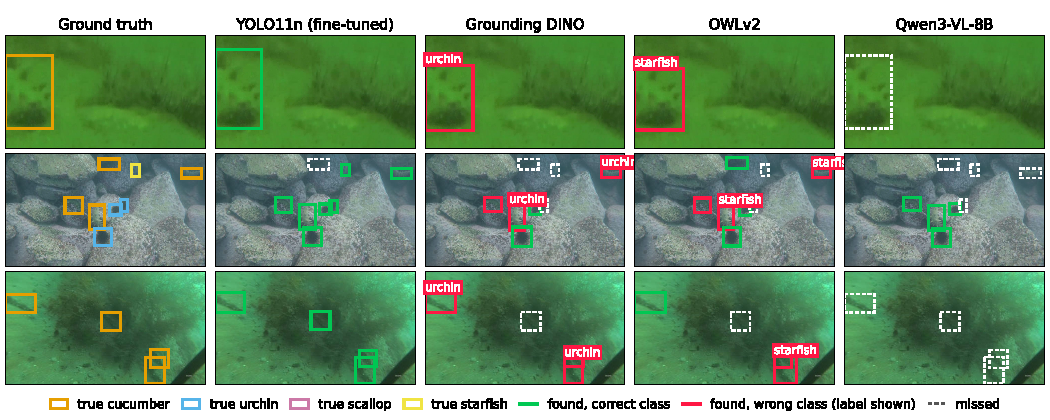
\includegraphics[width=\textwidth]{fig_examples.pdf}
\caption{Three DUO test images, cropped around their objects. The left column shows the true objects, colored by class. Every other column shows, for each true object, the model's best-overlapping box among the image's 100 highest-scoring boxes: green if the box carries the correct class, red with the assigned label if not (repeated labels on overlapping boxes are shown once), and a dashed outline if no box overlaps the object with IoU $\geq$ 0.5. This is the per-object view used in Section~\ref{sec:misnamed}, not the output at a fixed confidence threshold. Both open-vocabulary detectors box the sea cucumbers but call them sea urchins (Grounding DINO) or starfish (OWLv2); Qwen3-VL-8B names some sea cucumbers and misses others. Images from DUO \citep{liu2021duo}, CC BY 4.0.}
\label{fig:examples}
\end{figure*}

Robots that harvest or survey benthic animals such as sea cucumbers, sea urchins and scallops must detect each animal and know its species before acting on it. Training a detector for such a task requires labeled underwater images, which are costly to collect and annotate. Open-vocabulary detectors \citep{li2022glip,liu2024grounding,minderer2023scaling} and vision-language models (VLMs) that output boxes \citep{bai2025qwen25vl,bai2025qwen3vl} offer an alternative: they receive the class names as text and need no task-specific training.

Zero-shot detection is known to degrade outside web imagery. Roboflow100-VL reports large drops for Grounding DINO and Qwen2.5-VL across 100 datasets \citep{robicheaux2025rf100vl}, and VLM detectors recall few objects even on COCO \citep{fu2026wedetect}. These results establish \emph{that} zero-shot models fall short, not \emph{why}. A low average precision (AP) can come from missing the objects, from finding them but assigning the wrong class, or from evaluation choices that penalize a model's output format. The three causes call for different remedies: better localization, a better link between names and appearance, or a different evaluation.

We separate these causes on DUO \citep{liu2021duo}, an established underwater detection benchmark built from robot-picking contests, with four classes: sea cucumber, sea urchin, scallop and starfish. We compare six detectors fine-tuned on DUO with two open-vocabulary detectors (Grounding DINO and OWLv2) and three VLMs (Qwen2.5-VL-3B and -7B, Qwen3-VL-8B), all scored with the COCO protocol and paired bootstrap intervals. Beyond AP, we record for every ground-truth object whether any box covers it and whether such a box carries the correct class, and we compare models at a matched number of boxes. Our contributions are:
\begin{itemize}
\item \textbf{A controlled comparison} of fine-tuned and zero-shot detectors on an underwater robot-picking benchmark, with intervals for every comparison. The zero-shot gap is \dGap{} AP \dciGap{} between the weakest fine-tuned and the best zero-shot model (Section~\ref{sec:gap}).
\item \textbf{Evidence that zero-shot detectors find objects they cannot name, while VLMs name objects they do not find.} Grounding DINO and OWLv2 cover most sea cucumbers with a box but almost never label them correctly. A box-crop test confirms it: given the true box, each detector falls back to one default answer, and renaming the classes only changes which one. Given the box, the best VLM names \cropCucQwenVL\% of sea cucumbers, although in full images it finds only \scFoundQwenVL\% of them (Figures~\ref{fig:examples}--\ref{fig:crops}, Sections~\ref{sec:misnamed} and~\ref{sec:crops}).
\item \textbf{Evidence that evaluation choices change the verdict.} Output decoding changes Grounding DINO's AP by more than the difference between the two open-vocabulary detectors; at a matched box budget, the VLM that AP ranks last matches the best detector in precision and exceeds it in recall, confirming underwater what \citet{li2025aerialmlm} observed for aerial images; and one prompt sentence decides whether Qwen2.5-VL answers at all, without changing its AP (Section~\ref{sec:choices}).
\end{itemize}
Our study covers one benchmark; Section~\ref{sec:discussion} discusses what this allows us to conclude.

\section{Related Work}

\paragraph{Underwater detection benchmarks.}
DUO \citep{liu2021duo} re-annotates images from the URPC robot-picking contests and the UDD dataset \citep{liu2022udd} with four classes and reports baselines of fine-tuned detectors. RUOD \citep{fu2023ruod} contains 14,000 images with ten classes. \citet{wille2026domain} show that underwater domain factors affect both annotation quality and detector accuracy. Work on these benchmarks almost always trains detectors on them; we ask what models that have never been trained on underwater boxes achieve, and why.

\paragraph{Zero-shot detection beyond web images.}
GLIP \citep{li2022glip} introduced the ODinW transfer benchmark, and Grounding DINO \citep{liu2024grounding} and OWLv2 \citep{minderer2023scaling} are widely used open-vocabulary detectors. Roboflow100-VL \citep{robicheaux2025rf100vl} shows that their zero-shot AP drops sharply across 100 domains, which include aquatic datasets. \citet{chhipa2024robustness} measure the robustness of such detectors under distribution shifts of COCO. On aerial images, \citet{tsourveloudis2026aerial} finds that semantic confusion, rather than localization, limits open-vocabulary detectors, based on how performance changes when the vocabulary is reduced. MarineDet \citep{liang2023marinedet} trains an open-vocabulary detector for marine objects. We provide per-object evidence for the distinction between localization and naming underwater, and show how the confusions depend on the class names.

\paragraph{VLMs as detectors.}
Qwen2.5-VL \citep{bai2025qwen25vl} and Qwen3-VL \citep{bai2025qwen3vl} output boxes as text. \citet{fu2026wedetect} report that such models predict only part of the objects in an image and rarely reject classes that are absent. UWBench \citep{zhang2025uwbench} evaluates VLMs on underwater understanding, including grounding of referring expressions. VLM boxes carry no confidence score, so AP, which ranks boxes by confidence, measures them at a single operating point. Roboflow100-VL finds that adding confidence scores from a separate image-text model raises the AP of Qwen2.5-VL and Gemini, and that the prompt style changes their accuracy \citep{robicheaux2025rf100vl}. \citet{li2025aerialmlm} find on aerial images that the advantage of conventional detectors over multimodal language models in mAP largely comes from confidence scores, and recommend confidence-free measures. We confirm this effect underwater with a matched box budget, where it reverses the AP ranking of a VLM and two detectors.

\paragraph{Error analysis.}
TIDE \citep{bolya2020tide} attributes lost AP to error types such as wrong class, poor localization and missed objects. Our per-object measures complement it by recording, for each object, localization and naming separately, independently of how a model ranks its boxes. Classifying the crops of regions is a common diagnostic of open-vocabulary recognition \citep{gu2022vild}; we apply it with ground-truth boxes to separate naming from finding.

\begin{table*}[t]
\centering
\small
\setlength{\tabcolsep}{4.5pt}
\begin{tabular}{llccccccc}
\toprule
 & & \multicolumn{5}{c}{Full test set (\nTestImages{} images)} & First 100 images & \\
\cmidrule(lr){3-7}\cmidrule(lr){8-8}
Model & COCO AP & AP (95\% CI) & AP$_{50}$ & AR$_{100}$ & Merged AP & Sea cuc.\ AP & AP (95\% CI) & ms/image \\
\midrule
\multicolumn{9}{l}{\textit{Fine-tuned on DUO}} \\
YOLOv8n & 37.3 & 0.624 [0.593, 0.655] & 0.824 & 0.741 & 0.700 & 0.608 & 0.606 [0.482, 0.669] & 10 \\
YOLO11n & 39.5 & 0.625 [0.595, 0.652] & 0.820 & 0.747 & 0.705 & 0.606 & 0.628 [0.508, 0.692] & 11 \\
YOLO11s & 47.0 & 0.674 [0.645, 0.701] & 0.859 & 0.770 & 0.730 & 0.669 & 0.656 [0.526, 0.707] & 15 \\
YOLO11m & 51.5 & 0.685 [0.654, 0.712] & 0.857 & 0.780 & 0.742 & 0.680 & 0.684 [0.541, 0.735] & 13 \\
YOLO11l & 53.4 & 0.690 [0.662, 0.716] & 0.863 & 0.780 & 0.744 & 0.690 & 0.691 [0.556, 0.739] & 15 \\
RT-DETR-L & 53.0 & 0.669 [0.639, 0.695] & 0.849 & 0.774 & 0.718 & 0.666 & 0.692 [0.557, 0.742] & 21 \\
\midrule
\multicolumn{9}{l}{\textit{Zero-shot detectors}} \\
Grounding DINO & -- & 0.090 [0.067, 0.114] & 0.151 & 0.360 & 0.136 & 0.004 & 0.078 [0.048, 0.138] & 252$^\ddagger$ \\
OWLv2 & -- & 0.099 [0.088, 0.111] & 0.183 & 0.190 & 0.151 & 0.001 & 0.107 [0.078, 0.140] & 328 \\
\midrule
\multicolumn{9}{l}{\textit{Zero-shot VLMs}} \\
Qwen2.5-VL-3B & -- & 0.000 [0.000, 0.000] & 0.000 & 0.000 & 0.000 & 0.000 & 0.000 [0.000, 0.000] & 200 \\
Qwen2.5-VL-7B & -- & 0.013 [0.009, 0.018] & 0.024 & 0.021 & 0.016 & 0.004 & 0.018 [0.006, 0.034] & 632 \\
Qwen3-VL-8B & -- & \multicolumn{5}{c}{not run on the full test set} & 0.054 [0.043, 0.087] & 15{,}918 \\
\bottomrule
\end{tabular}
\caption{Detection results on the DUO test set (COCO protocol, pycocotools). Intervals are 95\% paired bootstrap intervals over test images. COCO AP is the published value for the fine-tuned architectures (Ultralytics). Merged AP treats all four classes as one, so a box counts regardless of its label. Qwen3-VL-8B was run only on the first 100 test images; the last column compares all models on those images. VLM boxes carry no confidence score and are all scored 1.0. Time per image on one RTX 5090: for the fine-tuned detectors, the median over 200 test images processed one at a time on an idle GPU, including pre- and post-processing; for the zero-shot models, wall-clock time over the whole run, including image loading. $^\ddagger$Grounding DINO shared the GPU with another job, so its time is an upper bound. Qwen2.5-VL is fast because it mostly returns an empty answer.}
\label{tab:main}
\end{table*}


\section{Experimental Setup}
\label{sec:setup}

\paragraph{Benchmark.}
DUO \citep{liu2021duo} contains 7,782 underwater images with the official split of 6,671 training and \nTestImages{} test images. The test set has \nTestObjects{} objects: \nSeaUrchin{} sea urchins (\shareSeaUrchin\%), \nStarfish{} starfish, \nSeaCucumber{} sea cucumbers and \nScallop{} scallops; \nImagesWithObjects{} test images contain at least one object. COCO AP averages over classes, so the three rarer classes weigh as much as sea urchins. The test set is used only for final scoring.

\paragraph{Fine-tuned detectors.}
YOLOv8n \citep{jocher2023yolov8}, YOLO11n/s/m/l \citep{jocher2024yolo11} and RT-DETR-L \citep{zhao2024rtdetr} start from COCO-pretrained weights and are trained with one recipe (Ultralytics 8.4.60): 640-pixel input, 40 epochs, batch size 8, seed 17. We hold out 10\% of the training split (667 images) to select the checkpoint. Training takes \trainMinMinutes--\trainMaxMinutes{} minutes per model on one RTX 5090 GPU. These detectors represent what a robot builder with labeled data would use.

\paragraph{Zero-shot models.}
We use Grounding DINO base \citep{liu2024grounding}, OWLv2 base \citep{minderer2023scaling}, Qwen2.5-VL-3B and -7B Instruct \citep{bai2025qwen25vl} and Qwen3-VL-8B Instruct \citep{bai2025qwen3vl}, run with Hugging Face Transformers 4.57.6 \citep{wolf2020transformers}. Grounding DINO receives the text prompt ``sea cucumber. sea urchin. scallop. starfish.''; OWLv2 receives one query per class, ``a photo of a $\langle$class$\rangle$''. The VLMs receive the image and the prompt
\begin{quote}\small
Detect every sea cucumber, sea urchin, scallop, starfish in this underwater image. Answer with JSON only: a list of objects, each \{"bbox\_2d": [x1, y1, x2, y2], "label": one of [sea cucumber, sea urchin, scallop, starfish]\}, with coordinates $\langle$coordinate phrase$\rangle$. Answer [] if there are none.
\end{quote}
where the coordinate phrase is ``in pixel coordinates of the image'' for Qwen2.5-VL and ``on a 0-1000 grid of the image (0,0 top-left, 1000,1000 bottom-right)'' for Qwen3-VL. Decoding is greedy with at most 1,536 new tokens, and box labels are matched to the four class names. Qwen3-VL-8B needs \secQwenVLmean{} seconds per image on average (median \secQwenVLmedian), against \secOWL{} for OWLv2. The prompt variations of Section~\ref{sec:choices} were run on the first 100 test images.

\paragraph{Scoring.}
We report COCO AP (IoU 0.50--0.95), AP$_{50}$ and recall with up to 100 boxes (AR$_{100}$), computed with pycocotools \citep{lin2014coco}. Fine-tuned detectors keep boxes with confidence $\geq$ 0.001 (up to 300 per image), open-vocabulary detectors boxes with confidence $\geq$ 0.01. Grounding DINO is scored as in its own COCO evaluation: the score of a class is the mean probability over the text tokens of its name, and the 300 highest-scoring (box, class) pairs per image are kept. VLM boxes carry no score, so all are scored 1.0; boxes extending beyond the image are clipped. A VLM reply cut off at the token limit is kept up to the cut: Qwen3-VL-8B's reply was cut off on \nCutQwenVL{} of the \nTestImages{} test images, and all \nOutsideQwenVL{} of its boxes that lay outside an image came from such replies. Intervals are 95\% percentile intervals from 500 bootstrap resamples of the test images \citep{efron1994introduction}; for a difference, both models are scored on the same resamples.

\paragraph{Per-object measures.}
An object is \emph{found} if at least one of the image's 100 highest-scoring boxes, of any class, overlaps it with IoU $\geq$ 0.5, and \emph{named} if at least one such box also carries the object's class. For each found object we record the class of the box with the highest IoU. These shares do not depend on how boxes are ranked within the 100; Section~\ref{sec:misnamed} varies the number of boxes and the IoU threshold. \emph{Merged AP} is AP after relabeling all objects and boxes as one class, keeping one box per location with its highest score; it measures detection regardless of the label.

\paragraph{Box-crop naming test.}
To test naming when localization is given, each zero-shot model sees only the crop of one ground-truth box, enlarged by 10\% on each side and upscaled to at least 56 pixels on its shorter side, and must give its class. We use all \nCropsScallop{} test scallops and \nCropsOther{} randomly chosen test objects of each other class (seed 17), \nCrops{} crops in total. The VLMs are asked ``This underwater image shows one object. Which one is it: sea cucumber, sea urchin, scallop, starfish? Answer with one of these names only.''; the open-vocabulary detectors answer with the class of their highest-scoring box in the crop, scored as above. We report the share of crops named correctly per class and its mean over classes, for which chance is 25\%, with bootstrap intervals over crops.

\paragraph{Matched box budget.}
A VLM returns a short, unranked list, while a detector returns a long, ranked one. To compare them at the same operating point, each detector keeps, on every image, its $k$ highest-scoring distinct boxes, where $k$ is the number of distinct boxes that Qwen3-VL-8B returned on that image; identical boxes count once for every model. All boxes then count equally, and we compute precision and recall at IoU $\geq$ 0.5 with the correct class. Because the budget comes from the VLM's own count, this comparison favors the detectors.

\section{Results}

\subsection{The Zero-Shot Gap}
\label{sec:gap}

Every zero-shot model is far below every fine-tuned detector (Table~\ref{tab:main}). The best zero-shot model, OWLv2, reaches \apOWL{} AP \ciOWL; the weakest fine-tuned detector, YOLOv8n, reaches \apYoloEightN{} \ciYoloEightN, a difference of \dGap{} \dciGap. Among the fine-tuned detectors the spread is small: YOLO11l exceeds YOLO11n by \dYoloSize{} \dciYoloSize. Among the VLMs, Qwen2.5-VL-3B returns no box at all, Qwen2.5-VL-7B reaches \apQSeven{}, and Qwen3-VL-8B reaches \apQwenVL{} \ciQwenVL. This confirms on an underwater robot-picking benchmark the general pattern reported by \citet{robicheaux2025rf100vl}. The remainder of this section asks where the gap comes from.

\subsection{Found but Misnamed}
\label{sec:misnamed}

\begin{figure}[t]
\centering
\includegraphics[width=\columnwidth]{fig_found_named.pdf}
\caption{Share of DUO test objects that are \emph{found} (light: some box among the image's 100 highest-scoring ones overlaps them with IoU $\geq$ 0.5) and \emph{named} (solid: such a box has the correct class), with 95\% bootstrap intervals. The fine-tuned YOLO11n finds and names almost every object. The zero-shot detectors find more than half of the sea cucumbers but name few of them; OWLv2 also names few of the scallops it finds.}
\label{fig:found}
\end{figure}

\begin{table}[t]
\centering
\small
\setlength{\tabcolsep}{2.8pt}
\begin{tabular}{lcccccc}
\toprule
 & & & \multicolumn{4}{c}{Label of best box (\%)} \\
\cmidrule(lr){4-7}
Model, names & Found & Named & Cuc. & Urch. & Scal. & Star. \\
\midrule
\multicolumn{7}{l}{Grounding DINO} \\
\quad common & 61 & 4 & 0 & 87 & 4 & 9 \\
\quad Latin & 52 & 34 & 27 & 15 & 13 & 46 \\
\multicolumn{7}{l}{OWLv2} \\
\quad common & 52 & 8 & 15 & 16 & 0 & 69 \\
\quad Latin & 52 & 0 & 0 & 8 & 0 & 92 \\
\midrule
YOLO11n, fine-tuned & 97 & 96 & 97 & 1 & 1 & 1 \\
Qwen3-VL-8B & 15 & 11 & 71 & 13 & 4 & 12 \\
\bottomrule
\end{tabular}
\caption{What happens to the \nSeaCucumber{} sea cucumbers in the DUO test set. Found: \% of objects overlapped (IoU $\geq$ 0.5) by any of the image's 100 highest-scoring boxes, of any class. Named: \% overlapped by such a box with the correct class. The right block gives the class of the best-overlapping box, as \% of the found sea cucumbers.}
\label{tab:seacucumber}
\end{table}

\begin{table}[!ht]
\centering
\small
\setlength{\tabcolsep}{2.8pt}
\begin{tabular}{llcccc}
\toprule
 & & \multicolumn{2}{c}{All objects} & \multicolumn{2}{c}{Sea cucumbers} \\
\cmidrule(lr){3-4}\cmidrule(lr){5-6}
Model & Boxes, IoU & Found & Named & Found & Named \\
\midrule
YOLO11n & 100, 0.5 & 96 & 95 & 97 & 96 \\
 & 10, 0.5 & 66 & 66 & 68 & 67 \\
 & 100, 0.7 & 86 & 86 & 89 & 89 \\
Grounding DINO & 100, 0.5 & 69 & 59 & 61 & 4 \\
 & 10, 0.5 & 31 & 25 & 21 & 0 \\
 & 100, 0.7 & 55 & 47 & 49 & 4 \\
OWLv2 & 100, 0.5 & 62 & 50 & 52 & 8 \\
 & 10, 0.5 & 37 & 33 & 20 & 3 \\
 & 100, 0.7 & 43 & 35 & 31 & 5 \\
\bottomrule
\end{tabular}
\caption{Found and named shares (\%, full test set) when only the 10 highest-scoring boxes per image count, or with IoU $\geq$ 0.7. All 95\% bootstrap intervals are within $\pm$5 percentage points.}
\label{tab:sensitivity}
\end{table}



Figure~\ref{fig:examples} shows typical cases and Figure~\ref{fig:found} the totals. The fine-tuned YOLO11n finds \foundYoloN\% of all test objects and names \namedYoloN\%. Grounding DINO finds \foundGD\% \foundciGD{} and names \namedGD\% \namedciGD; OWLv2 finds \foundOWL\% \foundciOWL{} and names \namedOWL\% \namedciOWL. Both open-vocabulary detectors thus leave about a third of the objects without any overlapping box, and lose a further \lossNamingGD{} and \lossNamingOWL{} percentage points of objects to wrong labels. Because sea urchins make up \shareSeaUrchin\% of the objects and are mostly named correctly, these totals hide where naming fails.

\paragraph{Sea cucumbers are found but almost never named.}
Grounding DINO covers \scFoundGD\% \scFoundciGD{} of the sea cucumbers with a box but names \scNamedGD\% \scNamedciGD{} correctly; OWLv2 covers \scFoundOWL\% \scFoundciOWL{} and names \scNamedOWL\% \scNamedciOWL{} (Table~\ref{tab:seacucumber}). Their sea-cucumber AP is \scApGD{} and \scApOWL{}, against \scApYoloN{} for YOLO11n. The wrong labels are systematic: of the \scFoundNGD{} sea cucumbers that Grounding DINO finds, it labels \scUrchinGD{} as sea urchins, and OWLv2 labels \scStarOWL{} of its \scFoundNOWL{} as starfish. Similar confusions affect other classes. Of the starfish that Grounding DINO finds, \starAsUrchinGD{} are labeled sea urchins and \starAsStarGD{} starfish. Of the scallops that OWLv2 finds, \scalAsStarOWL{} are labeled starfish, \scalAsUrchinOWL{} sea urchins and \scalAsScalOWL{} scallops.

\paragraph{Renaming moves the confusion.}
If the confusions came from unfamiliar common names, other names might remove them. They do not. With the Latin names ``holothurian'' and ``echinus'' in place of ``sea cucumber'' and ``sea urchin'', Grounding DINO names \scNamedGDlatin\% of the sea cucumbers correctly, but now labels \urchinAsHoloGDlatin{} sea urchins (\urchinAsHoloGDlatinPct\% of all sea urchins) as holothurians and \urchinAsScalGDlatin{} as scallops. Its AP does not improve: common minus Latin is \dLatinGd{} \dciLatinGd. OWLv2 names no sea cucumber correctly with the Latin name (\scNamedOWLlatin\%) and labels \scStarOWLlatin{} of them as starfish; its AP is slightly lower with Latin names (common minus Latin \dLatinOwl{} \dciLatinOwl). The class that a found object receives thus depends on the wording of the class list more than on the object's appearance.

\paragraph{Naming explains much of the gap, not all of it.}
Merged AP, which ignores labels, rises from \apGD{} to \mgGD{} \mgciGD{} for Grounding DINO and from \apOWL{} to \mgOWL{} \mgciOWL{} for OWLv2, an increase of about half. It remains far below the merged AP of the fine-tuned detectors (\mgYoloEightN--\mgYoloL). The open-vocabulary detectors therefore also box fewer objects than the fine-tuned ones and rank their correct boxes lower. The naming failure is robust to the measurement: with only the ten highest-scoring boxes per image, or with IoU $\geq$ 0.7, the share of sea cucumbers named correctly is \scNamedTopTenGD\% and \scNamedIouSeventyGD\% for Grounding DINO and \scNamedTopTenOWL\% and \scNamedIouSeventyOWL\% for OWLv2 (Table~\ref{tab:sensitivity}). Fewer boxes or a stricter IoU lower all shares, but the gap between found and named sea cucumbers remains.

\paragraph{The VLMs fail differently.}
Qwen3-VL-8B finds \foundQwenVL\% \foundciQwenVL{} of all objects and names \namedQwenVL\% \namedciQwenVL. For sea cucumbers it finds only \scFoundQwenVL\% \scFoundciQwenVL, so for this class it mostly misses rather than misnames; Section~\ref{sec:crops} shows that it can name most of them when given the box. Qwen2.5-VL-7B finds \foundQSeven\% of all objects because it rarely returns any box (Section~\ref{sec:prompt}).

\begin{figure*}[t]
\centering
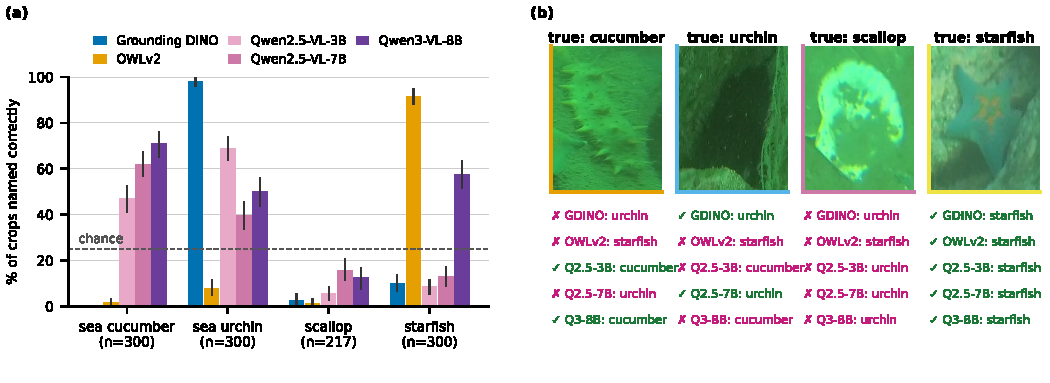
\includegraphics[width=\textwidth]{fig_crops.pdf}
\caption{Box-crop naming test. (a) Share of crops named correctly when each model sees only the crop of a true box, with 95\% bootstrap intervals; the dashed line marks chance. (b) One random crop per class (seed 17, among crops at least 150 pixels on the shorter side) with each model's answer: GDINO is Grounding DINO, Q2.5-3B and Q2.5-7B are Qwen2.5-VL-3B and -7B, Q3-8B is Qwen3-VL-8B. Images from DUO \citep{liu2021duo}, CC BY 4.0.}
\label{fig:crops}
\end{figure*}

\subsection{Naming When the Box Is Given}
\label{sec:crops}

\begin{table}[!ht]
\centering
\small
\setlength{\tabcolsep}{2.2pt}
\begin{tabular}{lcccccc}
\toprule
Model & Cuc. & Urch. & Scal. & Star. & Mean & Most frequent \\
\midrule
Grounding DINO & 0 & 98 & 3 & 10 & 28 & urch. 95\% \\
\quad Latin names & 88 & 5 & 7 & 13 & 28 & holot. 88\% \\
OWLv2 & 2 & 8 & 1 & 92 & 26 & star. 91\% \\
\quad Latin names & 25 & 7 & 3 & 76 & 28 & star. 65\% \\
Qwen2.5-VL-3B & 47 & 69 & 6 & 9 & 33 & urch. 57\% \\
Qwen2.5-VL-7B & 62 & 40 & 16 & 13 & 33 & cuc. 59\% \\
Qwen3-VL-8B & 71 & 50 & 12 & 58 & 48 & cuc. 52\% \\
\bottomrule
\end{tabular}
\caption{Box-crop naming test: \% of crops named correctly per class (cucumber, urchin, scallop, starfish) and the mean over classes; chance is 25\%. Per-class 95\% bootstrap intervals are within $\pm$6 points, intervals of the mean within $\pm$3. The last column gives the answer a model gives most often over all crops, and its share (holot.\ = holothurian).}
\label{tab:crops}
\end{table}


The box-crop test removes localization from the task (Figure~\ref{fig:crops} and Table~\ref{tab:crops}, which also gives the Latin-name results). Both open-vocabulary detectors are close to chance: their mean accuracy over the four classes is \cropGD\% \cropciGD{} for Grounding DINO and \cropOWL\% \cropciOWL{} for OWLv2. Each falls back to one answer: Grounding DINO calls \cropDefaultGD\% of all crops ``sea urchin'' and names \cropCucGD\% of the sea cucumbers, and OWLv2 calls \cropDefaultOWL\% of all crops ``starfish''. These are the same confusions as in full images (Table~\ref{tab:seacucumber}), so the detectors fail to name these classes even when localization is given. With Latin names, Grounding DINO's default answer switches to ``holothurian'' (\cropDefaultGDlatin\% of all crops): it now names \cropCucGDlatin\% of the sea cucumbers but only \cropUrchGDlatin\% of the sea urchins, and its mean accuracy stays at \cropGDlatin\% \cropciGDlatin. The answer follows the class names, not the object.

The VLMs name objects better when the box is given. Qwen3-VL-8B reaches a mean accuracy of \cropQwenVL\% \cropciQwenVL, \cropdGD{} percentage points \cropdciGD{} above Grounding DINO and \cropdQSeven{} points \cropdciQSeven{} above Qwen2.5-VL-7B, and names \cropCucQwenVL\% of the sea cucumbers. In full images, however, it found only \scFoundQwenVL\% of the sea cucumbers (Section~\ref{sec:misnamed}). Its main failure is therefore finding the objects, the opposite of the open-vocabulary detectors. Scallops remain hard for every model: no model names more than \cropScalMax\% of them.

\subsection{Evaluation Choices Change the Verdict}
\label{sec:choices}

\begin{table}[t]
\centering
\small
\setlength{\tabcolsep}{3pt}
\begin{tabular}{lc}
\toprule
Setting & Value (95\% CI) \\
\midrule
\multicolumn{2}{l}{\textit{(a) Grounding DINO decoding (DUO AP)}} \\
Own scoring $-$ phrase decoding & +0.042 [0.032, 0.053] \\
OWLv2 $-$ Grounding DINO & +0.009 [$-$0.015, 0.031] \\
\midrule
\multicolumn{2}{l}{\textit{(b) VLM prompt, $\Delta$AP on DUO (first 100 images)}} \\
\multicolumn{2}{l}{\quad no ``Answer []'' / one class per prompt:} \\
\quad Qwen2.5-VL-3B & +0.017 / +0.000 \\
\quad Qwen2.5-VL-7B & +0.000 / +0.018 \\
\quad Qwen3-VL-8B & $-$0.006 / +0.010 \\
\midrule
\multicolumn{2}{l}{\textit{(c) Qwen3-VL-8B minus Grounding DINO}} \\
DUO AP & $-$0.043 [$-$0.064, $-$0.016] \\
DUO P / R, matched boxes & +0.112 / +0.130 \\
RUOD AP (subset) & $-$0.061 [$-$0.070, $-$0.036] \\
RUOD P / R, matched boxes & +0.177 / +0.226 \\
\midrule
\multicolumn{2}{l}{\textit{(d) Qwen3-VL-8B minus OWLv2}} \\
DUO AP & $-$0.051 [$-$0.061, $-$0.040] \\
DUO P / R, matched boxes & $-$0.001 / +0.061 \\
RUOD AP (subset) & $-$0.009 [$-$0.019, 0.017] \\
RUOD P / R, matched boxes & +0.121 / +0.155 \\
\bottomrule
\end{tabular}
\caption{Evaluation choices. (a) The same Grounding DINO outputs scored as in its own COCO evaluation or through phrase decoding. (b) Change in AP when the sentence ``Answer [] if there are none'' is removed, or when the four classes are asked for one at a time (intervals in the text). (c, d) P, R: precision and recall. At a matched box budget (each detector keeps as many boxes per image as the VLM returned, all counting equally; IoU $\geq$ 0.5, correct class) the VLM matches or exceeds them; at IoU $\geq$ 0.75 its advantage shrinks (Section~\ref{sec:choices}). Differences are Qwen3-VL-8B minus the detector.}
\label{tab:choices}
\end{table}

\begin{table*}[t]
\centering
\small
\begin{tabular}{lcccc}
\toprule
Model & AP (95\% CI) & Precision (95\% CI) & Recall (95\% CI) & Boxes/image \\
\midrule
Qwen3-VL-8B & 0.048 [0.043, 0.056] & 0.349 [0.327, 0.374] & 0.402 [0.382, 0.424] & 10.9 \\
OWLv2 & 0.099 [0.088, 0.111] & 0.349 [0.323, 0.377] & 0.341 [0.321, 0.360] & 9.2 \\
Grounding DINO & 0.090 [0.067, 0.114] & 0.236 [0.220, 0.252] & 0.273 [0.256, 0.289] & 10.9 \\
YOLO11n (fine-tuned) & 0.625 [0.595, 0.652] & 0.558 [0.525, 0.591] & 0.624 [0.594, 0.653] & 10.6 \\
\midrule
Qwen3-VL-8B $-$ OWLv2 & $-$0.051 [$-$0.061, $-$0.040] & $-$0.001 [$-$0.016, 0.016] & +0.061 [0.048, 0.076] & \\
Qwen3-VL-8B $-$ G.\ DINO & $-$0.043 [$-$0.064, $-$0.016] & +0.112 [0.099, 0.127] & +0.130 [0.117, 0.144] & \\
\bottomrule
\end{tabular}
\caption{Ranking by AP against ranking at a matched box budget (full test set). AP uses each model's full ranked output. For precision and recall (IoU $\geq$ 0.5, correct class), each detector keeps on every image only as many of its highest-scoring distinct boxes as Qwen3-VL-8B returned there, and all boxes count equally. The last two rows give Qwen3-VL-8B minus the detector, with 95\% paired bootstrap intervals.}
\label{tab:budget}
\end{table*}



\paragraph{Output decoding.}
The Hugging Face pipeline turns each Grounding DINO box into a text phrase, which must then be matched to a class name. On DUO, \pctUnmatchedText\% of these phrases (\nUnmatchedText{} of \nBoxesText) match no class, for example ``seachin'', a fragment of ``sea urchin'', or ``sea urchin starfish'', which names two classes, and such boxes are lost. Scoring the same forward pass as in Grounding DINO's own COCO evaluation, which reads class scores directly from the token outputs, raises AP from \apGDtext{} to \apGD{}, by \dDecoding{} \dciDecoding{} (Table~\ref{tab:choices}a). This exceeds the difference between OWLv2 and Grounding DINO, \dOwlGd{} \dciOwlGd, which is not significant. An evaluation that used the pipeline would conclude that OWLv2 is about twice as accurate as Grounding DINO.

\paragraph{VLM outputs without confidence scores.}
AP rewards ranking boxes by confidence. A VLM's boxes all score 1.0, so its AP reflects one operating point, whereas a detector's AP integrates over all thresholds. AP places Qwen3-VL-8B (\apQwenVL) below OWLv2 (\apOWL; difference \dOwlQwenFull{} \dciOwlQwenFull) and Grounding DINO (\apGD; difference \dGdQwenFull{} \dciGdQwenFull). At a matched box budget the ranking changes (Table~\ref{tab:budget}). Qwen3-VL-8B is more precise and recalls more than Grounding DINO: the differences are \bdPGD{} \bdciPGD{} in precision and \bdRGD{} \bdciRGD{} in recall. Against OWLv2, precision is the same (\bdPOWL{} \bdciPOWL) and recall is higher (\bdROWL{} \bdciROWL). OWLv2 returned fewer distinct boxes than Qwen3-VL-8B on some images, so it used \bBoxesOWL{} rather than \bBoxesQwenVL{} boxes per image. The VLM's lower AP therefore reflects mainly its missing confidence ranking, not boxes or labels worse than those of the detectors. Under the same budget, the fine-tuned YOLO11n reaches a precision of \bPYoloN{} and a recall of \bRYoloN, so all zero-shot models remain far behind. With the number of true objects in each image as the budget instead, precision and recall are \gtbPGD{} and \gtbRGD{} for Grounding DINO, \gtbPOWL{} and \gtbROWL{} for OWLv2, and \gtbPYoloN{} and \gtbRYoloN{} for YOLO11n.

\begin{figure}[!ht]
\centering
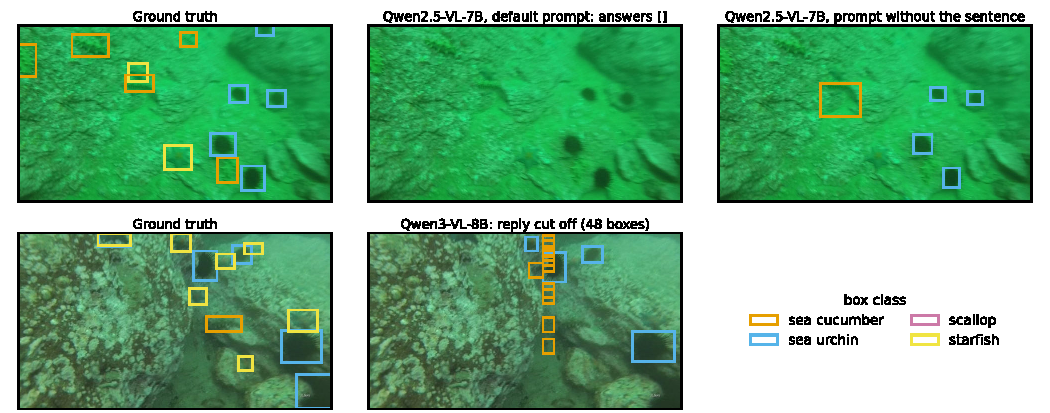
\includegraphics[width=\columnwidth]{fig_vlm_failures.pdf}
\caption{Two VLM failure modes on DUO test images. (a, b) With the default prompt, Qwen2.5-VL-7B answers with an empty list for an image with 12 objects; without the sentence ``Answer [] if there are none'' it returns boxes. (c, d) Qwen3-VL-8B keeps listing boxes, here a column of repeated sea-cucumber boxes, until its reply is cut off at the token limit. Boxes are drawn in the color of their class. Images from DUO \citep{liu2021duo}, CC BY 4.0.}
\label{fig:vlm}
\end{figure}

\paragraph{Prompt wording.}
\label{sec:prompt}
Our VLM prompt ends with ``Answer [] if there are none'', a common safeguard against invented boxes. With it, Qwen2.5-VL-3B returns an empty list on \nEmptyQThree{} of \nRepQThree{} test images and Qwen2.5-VL-7B on \nEmptyQSeven{} (\pctEmptyQSeven\%), although \nImagesWithObjects{} of the images contain objects. Without the sentence, run on the first 100 images, neither model returns an empty list. Yet AP barely moves (Table~\ref{tab:choices}b): the change is \dPromptSeven{} \dciPromptSeven{} for the 7B model and \dPromptThree{} \dciPromptThree{} for the 3B model. Without the sentence, \nCutQSevenNoEmpty{} of the 100 replies of the 7B model were cut off at the token limit by long lists of boxes. The sentence decides whether the model answers, not what it can see. Abstention rates of VLM detectors should therefore be reported together with the prompt that produced them. Figure~\ref{fig:vlm} shows an empty answer and, for Qwen3-VL-8B, a reply that lists boxes until it is cut off; such replies occurred on \nCutQwenVL{} of the \nTestImages{} test images, and Qwen3-VL-8B returned an empty list on \nEmptyQwenVL.

\subsection{What Does Not Explain the Gap}

\begin{table}[!ht]
\centering
\small
\setlength{\tabcolsep}{3.5pt}
\begin{tabular}{lcccccc}
\toprule
Model & Cls & Loc & Both & Dupe & Bkg & Miss \\
\midrule
YOLOv8n & 0.7 & 1.8 & 0.2 & 0.3 & 6.7 & 2.3 \\
YOLO11n & 0.7 & 2.2 & 0.2 & 0.3 & 6.5 & 2.1 \\
YOLO11s & 0.6 & 1.8 & 0.2 & 0.2 & 5.4 & 2.0 \\
YOLO11m & 0.6 & 1.7 & 0.2 & 0.1 & 5.7 & 1.8 \\
YOLO11l & 0.5 & 1.7 & 0.2 & 0.1 & 6.0 & 1.9 \\
RT-DETR-L & 0.5 & 1.8 & 0.2 & 0.1 & 5.3 & 3.1 \\
Grounding DINO & 19.5 & 2.2 & 0.2 & 0.3 & 5.6 & 3.6 \\
OWLv2 & 22.0 & 3.0 & 0.2 & 0.2 & 4.7 & 6.9 \\
Qwen2.5-VL-7B & 0.0 & 0.0 & 0.0 & 0.0 & 0.1 & 32.6 \\
Qwen3-VL-8B$^\dagger$ & 0.7 & 0.4 & 0.0 & 0.0 & 9.7 & 8.6 \\
\bottomrule
\end{tabular}
\caption{TIDE error breakdown: AP$_{50}$ points recovered by fixing each error type (Bolya et al.\ 2020). $^\dagger$First 100 images. The fixes are not additive, and the open-vocabulary detectors output several class labels for the same box, which inflates their Cls value; we therefore use TIDE only as supporting evidence.}
\label{tab:tide}
\end{table}


Halving the image-pixel budget of Qwen2.5-VL-7B changes its AP by \dResolution{} \dciResolution, which is not significant. Scale and model generation help: Qwen2.5-VL-7B exceeds the 3B model by \dSevenThree{} \dciSevenThree{}, and Qwen3-VL-8B exceeds Qwen2.5-VL-7B by \dQwenGenFull{} \dciQwenGenFull. Even so, the best VLM reaches less than a tenth of the AP of any fine-tuned detector on the same images. The TIDE error breakdown \citep{bolya2020tide} in Table~\ref{tab:tide} is consistent with these findings but less specific: boxes on background (Bkg) cost the fine-tuned detectors most, wrong classes (Cls) the open-vocabulary detectors, and missed objects (Miss) Qwen2.5-VL-7B.

\section{Discussion}
\label{sec:discussion}

\paragraph{Implications for robots.}
A picking robot acts on the class: a sea cucumber taken for a sea urchin leads to the wrong action. Our results indicate that current zero-shot detectors can propose where many objects are, since they cover most of them with some box, but cannot be relied on to say what the objects are: given the true box, they fall back to one default answer. The VLMs show the opposite pattern. Combining the two, zero-shot detector boxes as proposals and a VLM or a small classifier trained on a few labeled examples for naming, is a natural next step that we have not tested. Speed matters as well: the fine-tuned detectors need \msYoloMin--\msYoloMax{} ms per image, against \secQwenVLmean{} s on average for Qwen3-VL-8B (Table~\ref{tab:main}). Detectors fine-tuned on the benchmark remain the reliable option: they find almost every object, name \namedOfFoundMinYoloN--\namedOfFoundMaxYoloN\% of the objects they find correctly in every class (YOLO11n), and train in under three hours on one GPU.

\paragraph{Implications for evaluation.}
Our results suggest four reporting practices for zero-shot detection. First, state how an open-vocabulary detector's output is turned into classes, because decoding alone changed Grounding DINO's AP by more than the gap between two models. Second, as \citet{li2025aerialmlm} also recommend, compare VLMs with detectors with confidence-free measures, for example at a matched box budget, in addition to AP. Third, report the prompt with abstention rates, because one sentence switched Qwen2.5-VL between answering and not answering. Fourth, report per-class found and named shares, which separate localization from naming where AP does not.

\paragraph{Limitations.}
We study one benchmark, so we cannot show that the specific confusions generalize; the similar conclusion of \citet{tsourveloudis2026aerial} on aerial images suggests that the pattern is broader. Each model was prompted with one template, apart from the prompt variations of Section~\ref{sec:choices}. The found criterion is generous, as it accepts any of 100 boxes per image, although the naming failure persists with 10 boxes or a stricter IoU. The box-crop test removes the context around an object, which may help or hurt naming, and the open-vocabulary detectors answer it through their box scores, which is one of several possible ways to use them as classifiers. The shared word ``sea'' in two class names may contribute to Grounding DINO's bias toward ``sea urchin''; the Latin names, which share no word, shift the bias, which is consistent with a text-side effect but does not prove it. We did not check DUO's official split for images shared between training and test; such duplicates would inflate the fine-tuned detectors' scores but not the zero-shot results. Finally, underwater annotations are imperfect \citep{wille2026domain}. Annotation errors affect the fine-tuned detectors as well, yet these name nearly every object they find, so annotation errors alone cannot explain the zero-shot confusions.

\section{Conclusion}

On an established underwater robot-picking benchmark, zero-shot open-vocabulary detectors and VLMs fall far short of small fine-tuned detectors. The two kinds of model fail in different ways. The open-vocabulary detectors place boxes on most objects but label them according to the wording of the class list; given the true box, each falls back to one default answer. The VLMs name objects better when given the box but find fewer of them. Output decoding and the use of AP for outputs without confidence scores change scores and rankings as much as the choice of model, and prompt wording decides whether a VLM answers at all. Comparisons of zero-shot perception for robots should therefore report per-object and matched-budget measures alongside AP.

\bibliography{references}

\end{document}
